\section{Normal form near $C_1$: possible solitary wave solutions}
Using \eqref{eq:linode}, the curve $C_1$, corresponding to $\lambda = 0, 0\pm i \omega$, is given by
\begin{equation}\label{eq:c1}
C_1 : { p = 0, q < 0 }
\end{equation}
Which implies
\begin{equation}
a_1 > c^2
\end{equation}

In order to investigate the possibility of a $ sech^2 $  homoclinic orbit in the neighborhood of $C_1$ and delocalized solitary
waves, we next compute the normal form near $C_1$ following the procedure in \cite{IA}.

Near $C_1$ the dynamics reduce to a 4-D Center Manifold \cite{IA}
Since all the eigenvalues are non-hyperbolic, the Center Manifold has the form (a nonlinear coordinate change \cite{IA})
\begin{equation} \label{eq:c1cm}
Y = A \zeta_0 + B \zeta_0 + C \zeta_+ + \bar{C} \zeta_- + \Psi(\epsilon,A,B,C,\bar{C})
\end{equation}

with  a corresponding four-dimensional normal form
\begin{subequations}\label{eq:c1nf}
\begin{eqnarray}
\frac{dA}{dz} &=& B \\ \label{eq:aq}
\frac{dB}{dz} &=& \bar{\nu} A + b_* A^2 + c_* \left|C\right|^2 \\ \label{eq:bq}
\frac{dC}{dz} &=& i d_0 C + i \bar{\nu} d_1 C + i d_2 A C \label{eq:cq}
\end{eqnarray}
\end{subequations}
Here $C$ is complex, $\bar{C}$ is the complex conjugate of $C$, $\epsilon, \zeta_0, \zeta_1$ are given previously and the two new
complex eigenvectors co-spanning the Center Manifold are
\begin{equation}
\zeta_\pm	 = \left< 1, \lambda_\pm, 2 q / 3, \frac{\lambda_\pm}{3} q\right>^T 
\end{equation}

Using \eqref{eq:bq} and \eqref{eq:c0nf}
\begin{equation}
\bar{\nu} = b \epsilon = -\frac{\epsilon}{q} 
\end{equation}

Also from the characteristic equation \eqref{eq:charlinear}, the two non-zero 
(imaginary) roots are 
\begin{equation}
\lambda^2 = \frac{ q + \sqrt{q^2 + 4 \epsilon } }{2} \approx q \textrm{ for } \epsilon \textrm{ small }
\end{equation}

Hence
\begin{equation}
\lambda = \pm i \sqrt{-q}, q < 0
\end{equation}

Matching this to the linear part of \eqref{eq:cq} ( which corresponds to the imaginary eigenvalues), $\lambda = i d_0 = i \sqrt{-q}$ or 
\begin{equation}
d_0 = \sqrt{-q}
\end{equation}


If we do a dominant balance argument after the change of variable $\epsilon = \sqrt{-3 \alpha}$ on the characteristic equation as $\lambda \rightarrow 0 $ then we find $d_1 = \frac{ \sqrt{-3 \alpha} }{18 \alpha^2 } $. Using $\alpha=q/3$ we find $d_1 = \frac{\sqrt{-q}}{2 q^2} $ .

The remaining undetermined coefficients  in the normal form are the 
coefficients $b_*,c_*$ and $d_2$ 
which correspond to the $A^2, |C|^2$ and $AC$ terms respectively. In 
order to determine them, we follow the same procedure as 
in Section 3 and compute $dY/dz$ is two distinct ways. We expand the
function $\Psi$ as
\begin{equation}\label{eq:psiexp2}
\Psi(\epsilon,A,B,C,\bar{C}) = \epsilon A \Psi_{1000}^1 + \epsilon B \Psi_{0100}^1 + A^2 \Psi_{2000}^0 + A B \Psi_{1100}^0 + A C \Psi_{1010}^0 + \epsilon C \Psi_{0010}^1 + \cdots 
\end{equation}
with subscripts denoting powers of $A$, $B$, $C$ and $\bar{C}$, respectively,
and the superscript is the power of $\epsilon$. In the first way,
$dY/dz$ is computed by taking the $z$ derivative of \eqref{eq:c1cm} ( 
using \eqref{eq:c1nf} and \eqref{eq:psiexp2}) and read off the coefficients
of $A^2, \|C\|^2, C \epsilon$ and $AC$ terms.

In the second way, $dY/dz$ is computed using 
\eqref{eq:c1cm} and \eqref{eq:psiexp2} in \eqref{eq:bilinear} 
(with $p=0$ on $C_1$ as given in \eqref{eq:c1})
and the coefficients of  $A$, $B$, $C$ and $\bar{C}$ are once
again read off.

Equating the coefficients of the corresponding terms in the two
separate expressions for $dY/dz$ yields the following two systems of equations:

\begin{subequations}
\begin{eqnarray}
\mathcal{O}(A^2): &		b_* \zeta_1 &= L_{0q} \Psi_{2000}^0 - G_{1,2}(\zeta_0,\zeta_0) \\
\mathcal{O}(\left|C\right|^2):&	c_* \zeta_1 &= L_{0q} \Psi_{0011}^0 -2 G_{1,2}(\zeta_+,\zeta_-) \label{eq:cstar} \\
\mathcal{O}(\epsilon C): &-\frac{i}{q} \left(d_1 \zeta_+ +  d_0 \Psi_{0010}^1\right) &= L_{0q} \Psi_{0010}^1 - G_{1,2}(\Psi_{0010}^1,\Psi_{0010}^1) \\
\mathcal{O}(A C): 	&i d_2 \zeta_+ + i d_0 \Psi_{1010}^0 &= L_{0q} \Psi_{1010}^0 - 2 G_{1,2}(\zeta_0,\zeta_+)  \label{eq:AC}
\end{eqnarray}
\end{subequations}
where we have used the fact that $G_1$ and $G_2$ are symmetric bilinear forms. Equation \eqref{eq:cstar} is decoupled and yields 
$ c_* = \frac{8}{c^2}\left( 2 a_3 - a_2 \right)$ for \eqref{eq:GPC1} and 
$ c_* = \frac{1}{c^2}\left( 16 a_3 + \frac{140}{3} a_5 \right)$ for \eqref{eq:GPC2}. The only coefficient left to determine is $d_2$ which we shall compute now. 

Using $\Psi_{1010}^0 = \left<x_1,x_2,x_3,x_4\right>^T$ in \eqref{eq:AC} implies 
\begin{subequations}
\begin{eqnarray}
i d_2 + i d_0 x_1 &=& x_2 \label{eq:gpc1one} \\
- d_0 d_2 + i d_0 x_2 &=& \frac{q}{3} x_1 + x_3 \label{eq:gpc1two} \\
\frac{2 i q}{3} d_2 + i d_0 x_3 &=& \frac{q}{3} x_2 + x_4  \label{eq:gpc1three} \\
- \frac{q}{3} d_0 d_2 + i d_0 x_4 &=& \frac{q}{3}\left(\frac{q}{3} x_1 + x_3 \right) - \frac{ 2 q}{c^2}\left(\frac{7}{2} a_3 - \frac{i}{3} d_0 a_2\right) \label{eq:gpc1four}
\end{eqnarray}
\end{subequations}
for \eqref{eq:GPC1} and
\begin{subequations}
\begin{eqnarray}
i d_2 + i d_0 x_1 &=& x_2 \label{eq:gpc2one} \\
- d_0 d_2 + i d_0 x_2 &=& \frac{q}{3} x_1 + x_3 \label{eq:gpc2two} \\
\frac{2 i q}{3} d_2 + i d_0 x_3 &=& \frac{q}{3} x_2 + x_4  \label{eq:gpc2three} \\
- \frac{q}{3} d_0 d_2 + i d_0 x_4 &=& \frac{q}{3}\left(\frac{q}{3} x_1 + x_3 \right) - \frac{2 q}{c^2}\left( \frac{7}{2} a_3 + \frac{32}{3} a_5\right) \label{eq:gpc2four}
\end{eqnarray}
\end{subequations}
for \eqref{eq:GPC2}

Using \eqref{eq:gpc1one} in \eqref{eq:gpc1two} , \eqref{eq:gpc1two} in \eqref{eq:gpc1four} and using these in \eqref{eq:gpc1three} yields 
$ d_2 = \frac{1}{c^2}\left( \frac{7}{2 \sqrt{-q} } a_3 - \frac{i}{3} a_2 \right)$ for \eqref{eq:GPC1}.
Similarly using \eqref{eq:gpc2one} in \eqref{eq:gpc2two} , \eqref{eq:gpc2two} in \eqref{eq:gpc2four} and using these in \eqref{eq:gpc2three}  yields
$ d_2 = \frac{1}{\sqrt{-q} c^2}\left( \frac{7}{2 } a_3 + \frac{32}{3} a_5 \right)$  for \eqref{eq:GPC2}. 

Therefore the normal form near $C_1$ is 
\begin{subequations}\label{eq:GPC1normal}
\begin{eqnarray} \label{eq:GPC1normalA}
\frac{dA}{dz} &=& B \\ 
\frac{dB}{dz} &=& -\frac{\epsilon}{q} A - b_* A^2 + \frac{1}{c^2}\left( \frac{7}{2 \sqrt{-q} } a_3 - \frac{i}{3} a_2 \right)  \left|C\right|^2 \\ \label{eq:GPC1normalB}
\frac{dC}{dz} &=& i \sqrt{-q} C - i \frac{\sqrt{-q} }{q^3} C\epsilon + i \frac{1}{c^2}\left( \frac{7}{2 \sqrt{-q} } a_3 - \frac{i}{3} a_2 \right)A C \label{eq:GPC1normalC}
\end{eqnarray}
\end{subequations}
for \eqref{eq:GPC1} and
\begin{subequations}\label{eq:GPC2normal}
\begin{eqnarray} \label{eq:GPC2normalA}
\frac{dA}{dz} &=& B \\ 
\frac{dB}{dz} &=& -\frac{\epsilon}{q} A - b_* A^2 + \frac{1}{c^2}\left( 16 a_3 + \frac{140}{3} a_5 \right)  \left|C\right|^2 \\ \label{eq:GPC2normalB}
\frac{dC}{dz} &=& i \sqrt{-q} C - i \frac{\sqrt{-q} }{q^3} C\epsilon + i \frac{1}{\sqrt{-q} c^2}\left( \frac{7}{2 } a_3 + \frac{32}{3} a_5 \right)A C \label{eq:GPC2normalC}
\end{eqnarray}
\end{subequations}
for \eqref{eq:GPC2}.

The dynamics inherent in \eqref{eq:GPC1normal}, \eqref{eq:GPC2normal} may be elucidated following the discussions of \cite{IA} ,\cite{IK}, \cite{Lombardi1} and\cite{Lombardi2}.
The two first integrals of \eqref{eq:c1nf}  are
\begin{equation}
K = \left| C \right|^2
\end{equation}
and
\begin{equation}\label{eq:H}
H = B^2 - \frac{2}{3} b_* A^3 - \bar{\nu} A^2 - 2 c_* K A
\end{equation}

Here, the appropriate coefficients $b_*, \bar{\nu}$ and $ c_*$, derived above, apply for \eqref{eq:GPC1} and \eqref{eq:GPC2}. 
Also, $c_*$ should be real, or $a_2$ must be zero in \eqref{eq:GPC1} for the following energy arguments to apply.


As a typical case, consider  the level curve $H=0$ of the energy-like first integral function $H$. In the $(A,B)$ phase plane,
this will compromise a homoclinic orbit. The intersection of $H=0$ with the $A$ axis occurs for $ \frac{2}{3} b_* A^2 - \bar{\nu}A - 2 c_* K = 0$ or
\begin{equation}
A_{\mp} = \frac{3}{4 b_*} \left[ \bar{\nu} \pm \sqrt{ \bar{\nu}^2 + \frac{16 b_* c_* K}{3} } \right]
\end{equation}

\begin{figure}[hh]
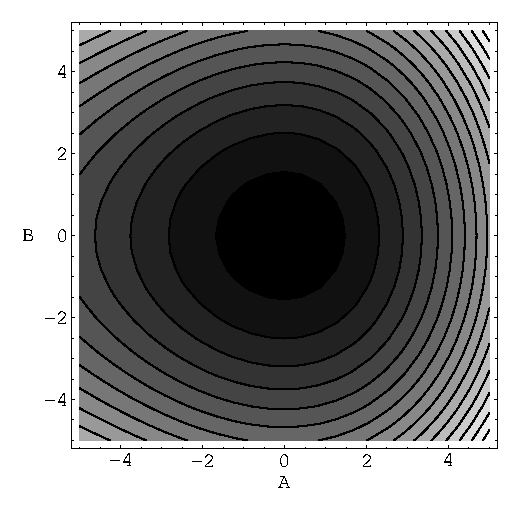
\epsfig{file=../homoclinic, scale=1.0}
\label{fig:homoclinic}
\caption{Level curves of \eqref{eq:H} corresponding to various values of H.}
\end{figure}

Note that $A_+ > 0, A_- < 0 $ for $b_* c_* > 0 $ and $b_* < 0$ as relevant for us. A general homoclinic orbit, homoclinic to $A_+$, is sketched
in Figure 1 where the flow direction is deduced from \eqref{eq:GPC1normalA} and \eqref{eq:GPC2normalA} for \eqref{eq:GPC1} and \eqref{eq:GPC2}, respectively.
For $K=\left|C\right|^2 = 0 $, the orbit is homoclinic to $A_+=0$. For small non-zero $\left|K\right|$, $ A_+ \sim - 2 c_* K / \bar{\nu}$, meaning that
oscillations at infinity are then very small in this case. For $K=0$ this corresponds to an orbit homoclinic to 0 for the normal form. This is indeed valid for
the normal form taken at any order. However this solution does not exist mathematically for the full original system, even though
one may compute its expansion in powers of the bifurcation parameter up to any order (see \cite{Lombardi1} and \cite{Lombardi2}). This is an example
of the famous challenging problem of asymptotics beyond any orders. Other solutions found on the normal form mainly persist under the perturbation from
higher order terms provided by the original system \cite{IK}. These solutions are delocalized waves and their existence in Region 2 is guaranteed
by the general theory for reversible systems in \cite{Lombardi1} and \cite{Lombardi2}. Also, as mentioned in Section 2, genuine solitary waves are found on isolated
curves in Region 2 of Figure 1 on which the oscillation amplitudes vanish. Since these are embedded in the sea of delocalized solitary waves and in the 
continuous spectrum, they are referred to as embedded solitons \cite{CMYK}. These will further be investigated in Region 2 subsequently using a mix of
exponential asymptotics and numerical shooting.


